\section{10. Жорданова диаграмма. Метод ее построения без поиска жорданова базиса. Теорема о единственности жордановой нормальной формы с точностью до перестановки клеток.}

\begin{definition}
    \textit{Жордановой диаграммой}, соответствующей Жордановой матрице $J$, называется набор точек на плоскости, изображающих вектора Жорданова базиса. При этом точка с координатой $(i, j)$ 
    изображает вектор $f_{ij}$ Жорданова базиса. Под каждым столбцом Жордановой диаграммы указывается соответствующее векторам этого 
    столбца собственные значения.
\end{definition}

\begin{example}
    Пусть $\phi$ имеет в некотором базисе следующую матрицу:
        \[A = \begin{pmatrix}
        \lambda & 1        & 0       & 0       & 0        & 0    &0    & 0\\
        0       & \lambda  & 1       & 0       & 0        & 0    &0    & 0\\
        0       & 0        & \lambda & 0       & 0        & 0    &0    & 0\\
        0       & 0        & 0       & \lambda & 1        & 0    &0    & 0\\
        0       & 0        & 0       & 0       & \lambda  & 0    &0    & 0\\
        0       & 0        & 0       & 0       & 0        & \mu  &1    & 0\\
        0       & 0        & 0       & 0       & 0        & 0    &\mu  & 0\\
        0       & 0        & 0       & 0       & 0        & 0    &0    & \nu
        \end{pmatrix}\]
        
    Четыре Жордановы клетки: порядков $2$ и $3$ с собственным значением $\lambda$, порядка $2$ с собственным значением $\mu$ и порядка $1$ с собственным значением $\nu$. 
    
    Такая матрица является Жордановой. Начнем выписывать Жорданов базис: $f_{11}$, $f_{12}$, $f_{13}$, $f_{21}$, $f_{22}$, $f_{31}$, $f_{32}$, $f_{41}$.
    
    В общем случае, если мы пишем Жорданов базис в виде $f_{ij}$, коэффициенты означают номер клетки и 
    номер вектора относительно данной клетки соответственно. Теперь вектор $f_{ij}$ можно сопоставить 
    точке на графике с координатами $(i, j)$. Если под каждым столбцом указать соответсвующие векторам столбца собственные значения, то полученный график называется Жордановой диаграммой.
    \begin{center}
        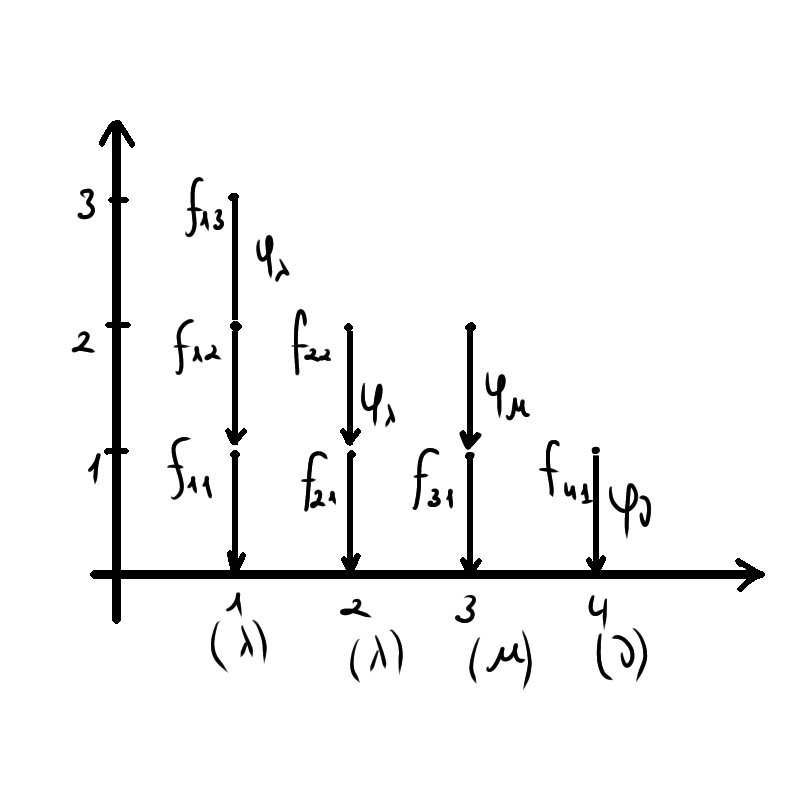
\includegraphics[width = 0.4\textwidth]{images/lec6_1.PNG}
    \end{center}
\end{example}

\begin{note}
    Столбцы не обязательно должны быть отсортированы в порядке невозрастания, диаграмма соотвествует 
    конкретной матрице и меняется при перестановке клеток местами.
\end{note}

\begin{proposition}[Свойства Жордановой диаграммы]~
    \begin{enumerate}
        \item Соответствие Жордановой матрицы $J$ и Жордановой диаграммы $J$ взаимно однозначно.
        \item Векторы Жордановой диаграммы, относящиеся к собственному значению $\lambda_i$, образуют базис 
        в корневом подпространстве $V^{\lambda_i}$.
        \item Если вектор $f_{ij}$ относится к собственному значению $\lambda_i$, 
        то он является корневым вектором, относящимся к $\lambda_i$ высоты $j$, 
        то есть $\phi_{\lambda_i}^j f_{ij} = \overline{0}$, но $\phi_{\lambda_i}^{j-1} f_{ij} \neq \overline{0}$.
        На высоте 1 в Жордановой диаграммы находятся собственные векторы оператора $\phi$.
        \item Если $f_{ij}$ относится к собственному значению $\lambda_{j}$, то $\phi_{\lambda_i} f_{ij} = f_{i(j-1)}$.
        %Нарисовать диаграмму со стрелочками вниз и нули на нижней линии.
        \item Каждый столбец в Жордановой диаграмме является изображением циклического подпространства для оператора $\phi_{\lambda_i}$. Общее число столбцов в Жордановой диаграмме $\displaystyle\sum_{i=1}^{k} geom(\lambda_i)$.
    \end{enumerate}
\end{proposition}

\begin{proposition}
    Пусть $\phi : V \to V$. Тогда справедливы следующие вложения:
    \begin{enumerate}
        \item $\ker \phi^0 \subseteq \ker \phi \subseteq \ker \phi^2 \subseteq \dots$
        \item $\im \phi^0 \supseteq \im \phi \supseteq \im \phi^2 \supseteq \dots$
    \end{enumerate}
    Причем обе цепочки стабилизируются за конечное число шагов.
\end{proposition}

\begin{proof}
    Индукция по $n \in \Z_{\geq 0}$:

    \begin{enumerate}
        \item База индукции: $\ker \phi^0 = \ker E = {\overline{0}} \subseteq \ker \phi \ \forall \phi$ и аналогично $\im \phi^0 = \im E = V \supseteq \im \phi \ \forall \phi$.
        \item Докажем, что $\ker \phi^n \subseteq \ker \phi^{n+1}$ (где $n \in \N$):
        Если $x \in \ker \phi^n$, тогда $\phi^n x = 0$ и $\phi ^{n + 1} x = \phi (\phi ^ n x) = \phi (\overline{0}) = \overline{0}$. \\
        Докажем теперь аналогичное вложение для образов: пусть $y \in \im \phi^{n + 1}$, тогда существует $x$, такой что $y = \phi^{n + 1} x = \phi^n(\phi(x)) = \phi^n z \in \im \phi^n$. Следовательно, $\im \phi^{n + 1} \subseteq \im \phi^n$.
    \end{enumerate}
\end{proof}

\begin{algorithm}[Построение Жордановой диаграммы]

    Покажем, как это использовать для нахождения Жордановой матрицы. Обозначим размерности ядер за $n_i$ соответственно: $\dim \ker \phi^i = n_i$. Выпишем для одного подпространства $U_{\lambda}$ все вложенные в него:
    \begin{eqnarray}  
        \{0\} \subseteq \ker \phi_{\lambda} = \langle f_{11}, f_{12}\rangle \subseteq \ker \phi_{\lambda}^2 
        = \langle f_{11}, f_{21}, f_{12}, f_{22} \rangle \subseteq \ker \phi_{\lambda}^3 = 
        \langle f_{11}, f_{21}, f_{12}, f_{22}, f_{13} \rangle, \\ (n_1 = 2, n_2 = 4, n_3 = 5).
    \end{eqnarray}
    Тогда число точек в Жордановой диаграмме на высоте $j$ равно $d_j = n_j - n_{j-1}$, откуда для нашего примера соответствующие $d$ равны $d_1 = 2-0=2, d_2 = 4-2=2, d_3 = 5-4=1$.
    
    Если в корневом пространстве $V^{\lambda}$ ввести обозначения $d_j$ - число векторов (точек) на высоте $j$, то $d_j = n_j - n_{j-1}$, где $n_0 = 0$, $n_k = \dim \ker (\phi - \lambda_i E)^k$.
    Это работает, потому что при применении оператора $j$ раз обнулятся все векторы на высоте не выше $j$, 
    тогда при применении на $1$ раз меньше обнулятся все, кто ниже, искомое количество - те, кто обнуляется при применении $j$ раз и не обнуляется при применении на 1 раз меньше.
    
    Строим ядра (и образы) до тех пор, пока они не стабилизируются (будут равны).
\end{algorithm}

\begin{theorem}[]
    Жорданова нормальная форма линейного оператора $\phi$ опеределена однозначно с точностью до перестановки Жордановых клеток, стоящих на главной диагонали. 
    Утверждение складывается из двух промежуточных:
    \begin{enumerate}
        \item Сумма порядков клеток, относящихся к собственному значению $\lambda_i$, не зависит от выбора Жорданова базиса.
        \item Для оператора $\phi$, имеющего единственное собственное значение, порядки Жордановых клеток определяются однозначно.
    \end{enumerate}
\end{theorem}

\begin{proof}~
    \begin{enumerate}
        \item  Зафиксируем Жорданов базис и корневое подпростарнство $V^{\lambda_i}$ и выберем все векторы Жорданова базиса, относящиеся к $\lambda_i$. Обозначим $V(\lambda_i) = \langle f_{ij} | f_{ij}$ относящиеся к $\lambda_i \rangle$. \\
        Пусть $l_i$ -- максимальный порядок Жордановых клеток Жордановой матрицы, отвечающих $\lambda_i$, $(J_k(\lambda_i) - \lambda_i \epsilon)^{l_i} = 0$. 
        Оператор нильпотентен и за несколько его применений все векторы базса обратятся в 0.
        Таким образом $(\phi - \lambda_i \epsilon)^{l_i} \vert_{V(\lambda_i)} = 0$.
        $\forall i V(\lambda_i) \subseteq V^{\lambda_i}$ -- так как все векторы аннулируются.
        \begin{enumerate}
            \item $V = V^{\lambda_1} \oplus V^{\lambda_2} \oplus \dots \oplus V^{\lambda_k}$.
            \item $V = V(\lambda_1) \oplus V(\lambda_2) \oplus \dots \oplus V(\lambda_k)$.
        \end{enumerate}
        По теореме о характеризации прямой суммы второе выражение является прямой суммой, а значит верны вложения и в обратную сторону(из соображений размерности).
        \item Пусть единственное собственное значение -- 0. Покажем, что размеры клеток в Жордановой нормальной форме определены однозначно. 
        Как было доказано на предыдущих лекциях, из того, что оператор нильпотентен, существует разложение в прямую сумму циклических подпространств.
        \begin{center}
            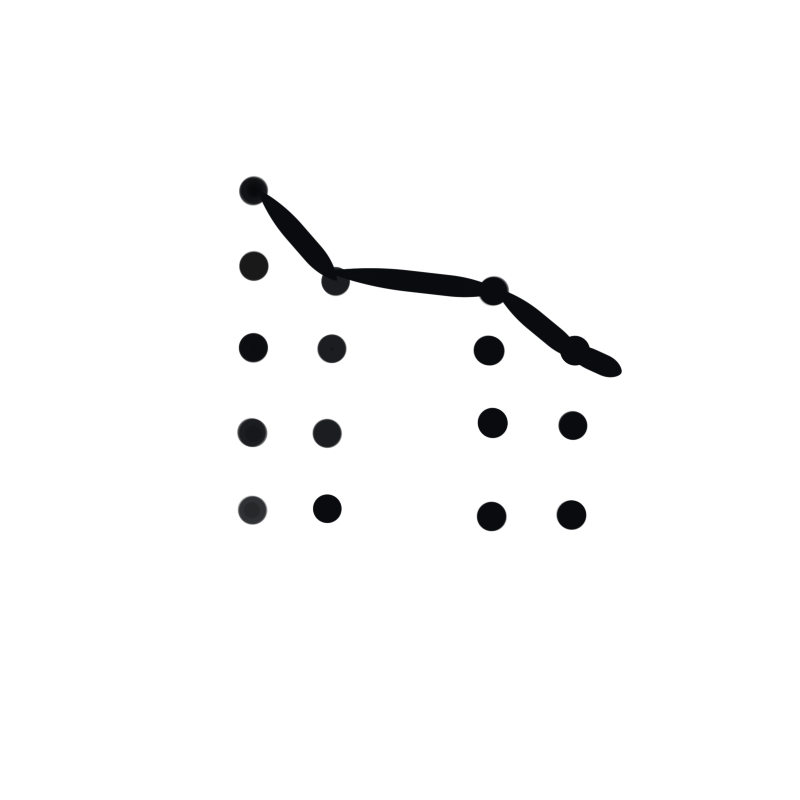
\includegraphics[width = 0.2\textwidth]{images/lec6_5.PNG}
        \end{center}
        Длины строк определены однозначно: $d_j = n_j - n_{j-1}$, $n_j = \dim \ker \phi^j$. Таким образом порядок клеток тоже можно определить однозначно.
    \end{enumerate}
\end{proof}